\documentclass[12 pt]{article}
\usepackage[margin = 1.0in, letterpaper]{geometry}
\usepackage{graphicx}
\usepackage{amsfonts, amsmath}
\usepackage{float}

\begin{document}

\title{The Digital Age, Fourier Transforms and Spectra}
\author{Eduardo Herrera}

\maketitle

\begin{abstract} 
It is crucial to sample at a rate such that one can resolve and
characterize the incoming signal. It is shown that at the nyquist rate
$v_{sig}=.5*v_{samp}$ one can resolve and use the detected signal, without the
alternatives of getting false data or wasting too many resources in
terms of memory which becomes costly. Power spectra
across frequency are used to help differentiate between to signals
when mixed together and hekp diffrentiate between the mixed waves and
`noise' made by them. Important results include the calculation of tones
from mixed signals and using fourier transforms to see the peaks of
signals at frequecies that vary a little. 

\end{abstract}

\section{Introduction}
In the larger scope of making important but slowly emerging dicoveries that could help
mankind better know their place and role in the universe, we must amke
use of our small-scale inventions.
Utilization of small chips programmed to make incredibly fast computations that
would not be practical for us to attempt by hand. Thanks to the wide variety
of chips with storage and processing power today and in the future, we
may be able to get to those grand discoveries faster. In the digital
lab, code and knowledge of computer components lead to a proper
understanding of digital sampling, Fourier Transforms (leading to power
spectrums) and mixing, all with application to the radio astronomy
field, especially when analyzing signals that could only be analyzed via
radio astronomy. In the first section of the lab we sample at
some fraction of a frequency to see what the minumum sample rate is to
get good data, while taking the least computer resources to get that
data. In the following section we mix two types of signals together and
analyze their power spectrums, although this may be misleading because
the power of the signal imput is not physical but shows a peak.
Finally we work with the ROACH to create a filter that can be
manipulated via coefficient inputs we can choose.

\section{Week  One: Sampling}

\subsection{Methods}
For the first week of the lab,  we needed to take control of the pulsar
and the oscillator and from there take samples at some $v_{sig}$ with
some constant sample frequency of $v_{samp}$ which was chosen to be 10
MHz. $v_{sig}$ was chosen so that it would increase in increments of
.1$v_{samp}$ for nine trials. From there we labeled our data points for
which the signal was sampled at, at time intervals set up by $v_{sig}$
this was done to test the Nyquist sampling rate. 

\subsection{Going to the Extremes}
Before our data for $v_{sig}$, there should be a check on the extremes
of Nyquist sampling, namely $v_{sig} = v_{samp}$ and
$\frac{v_{sig}}{v_{samp}} = large$. In the latter case, when we come
across this condition, our graph ends up looking like the figure below

\begin{figure}[H]
\center
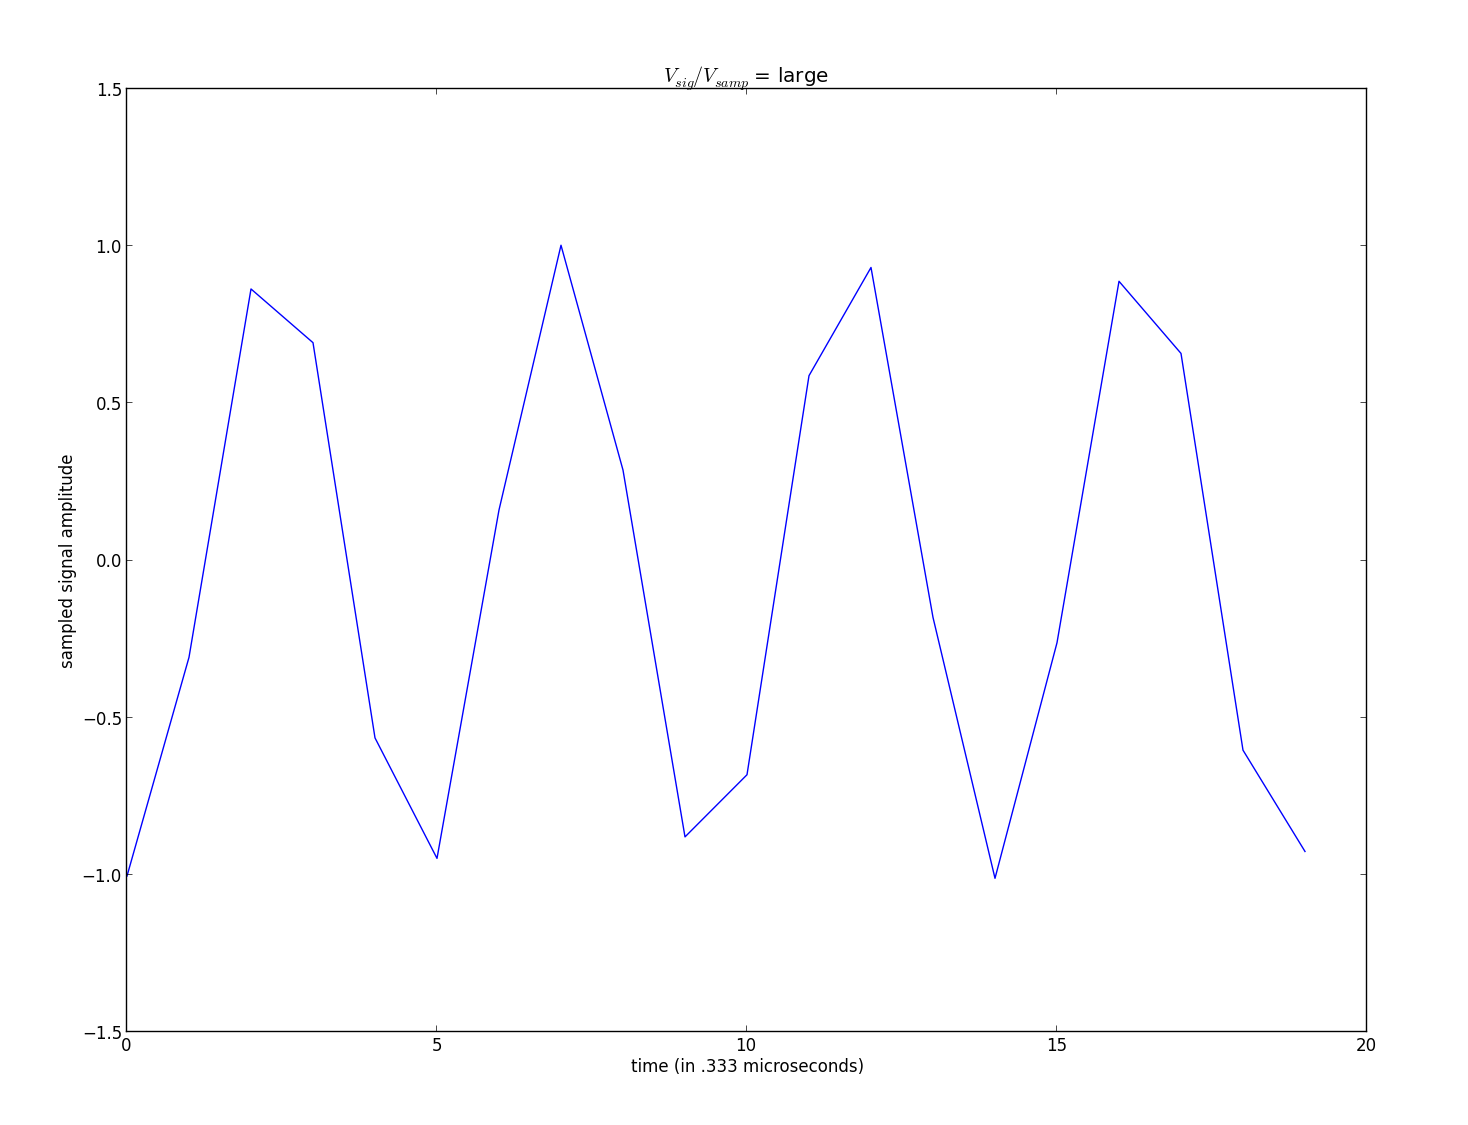
\includegraphics[scale=0.4]{vsigovervsamplarge.png}
\caption{The plot of $\frac{v_{sig}}{v_{samp}} = large$ for $v_{sig} =
  30 MHz$ and $v_{samp} = 500 Hz$.}
\label{signal equals the sampling rate}
\end{figure}
at this sampling rate, we see that since the ratio between the signal
and the sample frequency is so large, the data points taken are not
sufficient to recreate the wave because our sampling frequency is much
too slow to catch up with the maximum frequency and so we are left
unable to charecterize to above wave. 

For the case of $v_{sig} = v_{samp}$ my plot for the data did not come
out to a straight line as it was predicted it would, it is ommitted here
since it was an error on part of the equipment that it did not work. The
reason this plot would be a straight line is because the sampling
frequency would only sample at the period of the incoming signal,
resulting in just a horizontal line when connecting the dots, there is
no wave to analyze. 
\subsection{Nyquist Frequency}

Now to demostrate an understanding of the Nyquist frequency, there is a
graph below that gives the signal frequency in increments of .1 of the
sample frequency, and of interest is the fifth graph.

\begin{figure}[H]
\center
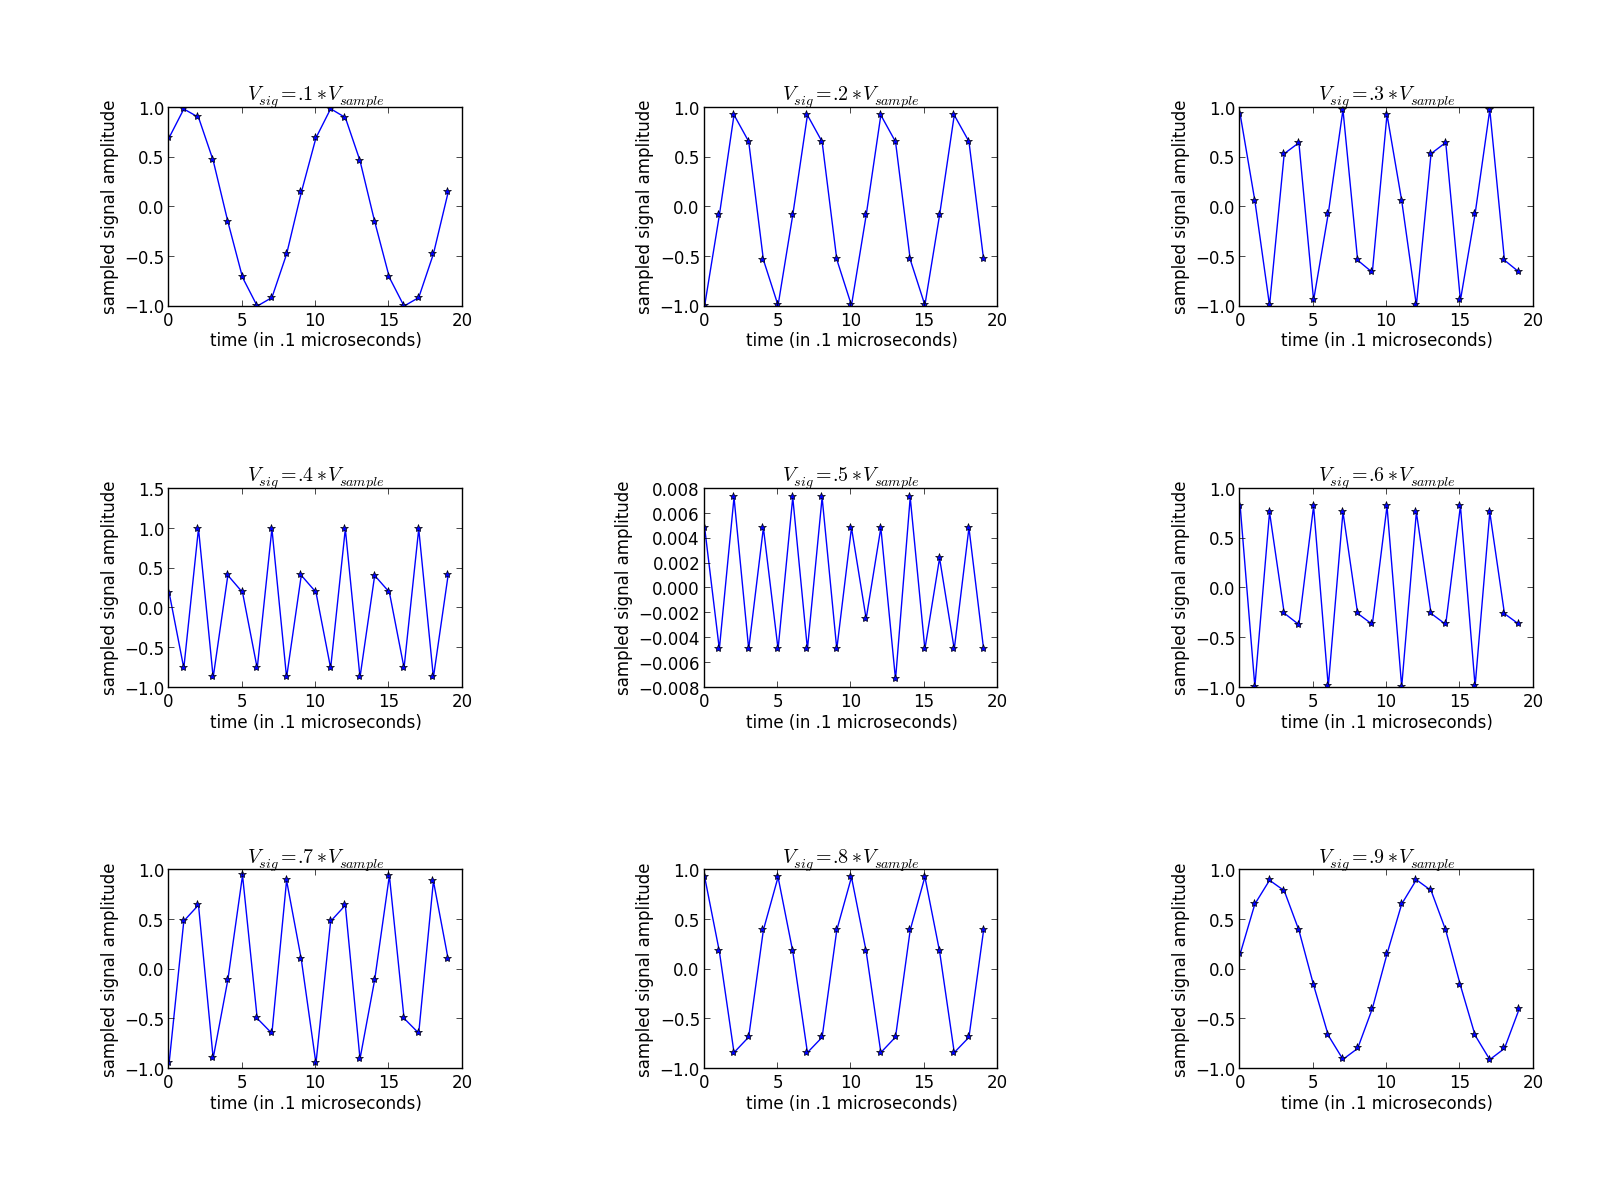
\includegraphics[scale=0.4]{Nyquiststar.png}
\caption{a series of plots demonstrating the declining effectives of
  sampling when you stray below the nyquist rate (at least twice the
  maximum frequency)}
\label{Nyquiststar}
\end{figure}
Here, we see the Nyquist criterion at work for a sampling frequency of
10 MHz, starting with the top left
corner, we see that the wave is accurately represented since many points
(represented by the starred data points) were able to be plotted along
the line of the signal and thus we get an accurate representation of the
wave. Looking at the top right plot we see now that the data points were
plotted at larger intervals of time (we see less of a curve on th
turning points of the signal), but overall, we can still characterize
the signal. One important plot to note is the fifth plot taken right at
the Nyquist sample rate. The reason the y-axis of this plot is different
from the rest is that the pulsar sampler couldn't easily do the sampling
at 10 Mhz, because of this, pulsar had to skip samples to simulate
sampling at that frequency (it usually samples at 20 Mhz). Aside from
these strange jump in the data, we see that at Nyquist sampling rate,
the wave is barely resolved at that signal frequency. Now once we get
past the fifth, we see that the next graphs look similar to the previous
graphs we have looked at, although this may seem that the data points
are still accurately representing the signal frequency, they aren't. The
signal frquency is going through more cycles, and the data points can't
accurately make a plot that represents that signal frquency. By the time
we reach the ninth plot, the signal frequency undergoes many cycles and
the data points were only able to record at a few points which
definitely does not reproduce the graph. The reason Nyquist's criterion
is preferred is because it is the best way to recreate an incoming
signal using the least amount of computation power, you could make it
more exact to the wavelength by making sure the sampling rate is higher
than the signal rate but that takes up more time and resources on the
computer than would be expcted since there are other devices that need
computers to function, all simultaneously.

\subsection{Power Spectrum}
Here, the spectrum of the previous 9 plots was Fourier transformed
 and then squared to get rid of complex numbers that were a product of
 the imaginary number in the exponential, together with a frequency and
 sample number, the plots now
 look like
 
\begin{figure}[H]
\center
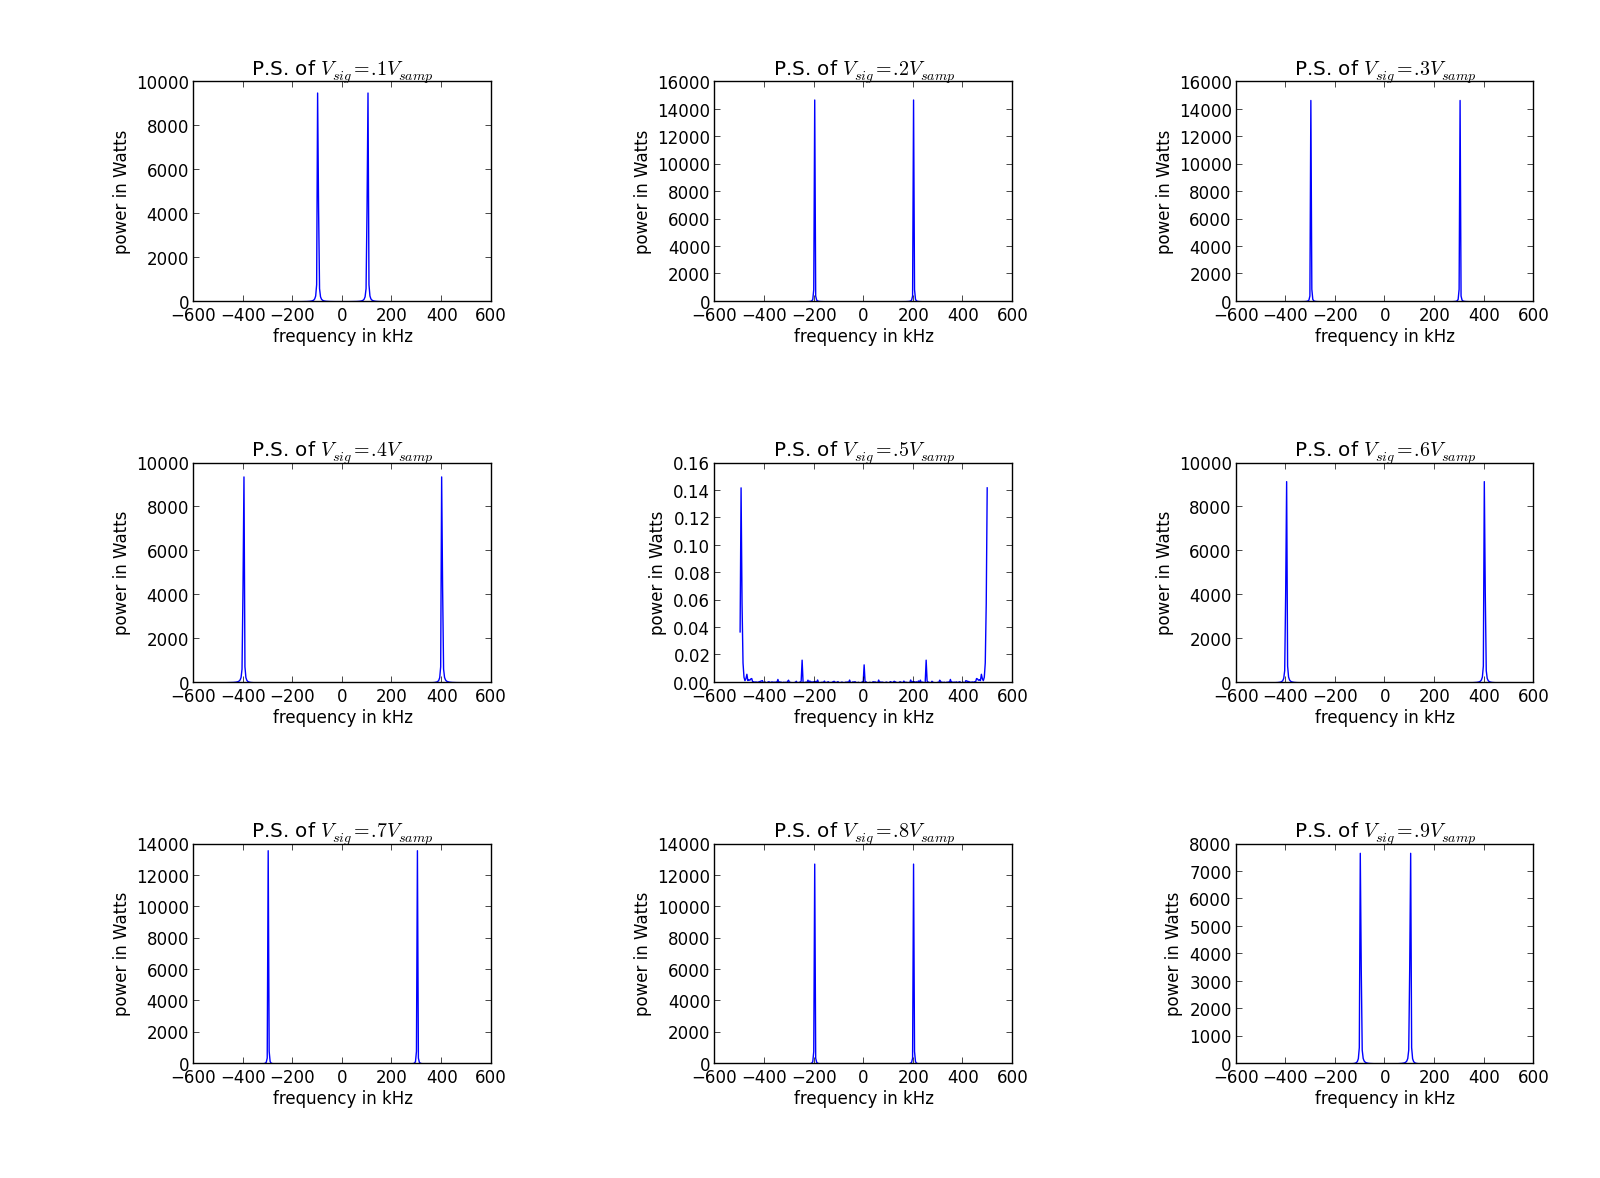
\includegraphics[scale=0.4]{DFTplots.png}
\caption{The DFT plots of our previous Nyquist plots}
\label{DFTplots}
\end{figure}

So these are the transfers to a power spectrum, and as we see, there are
two spikes, the one to the right represents the real part of the sine
wave while the second spike represents the imaginary part of the
wave. The reason that they pop up, is from the afroementioned Fourier
transform, the exponential term introduces a complex number which
becomes negative when i is squared, and so hence, two spkies
appear. There is also a pattern of the spikes getting further away from
eachother until the Nyquist criterion and then come back together as
ther start to violate that law. The place the spikes are at is
prortional to $v_{sig}$, being a fraction of the sample frequency. 

\subsection{Spectral Leakage}
Spectral leakage is represented by the following graphs which have all
been modified to show the leakage(by taking the log of the previous set
of plots), shown as the fringes along the curve
of the spikes. 

\begin{figure}[H]
\center
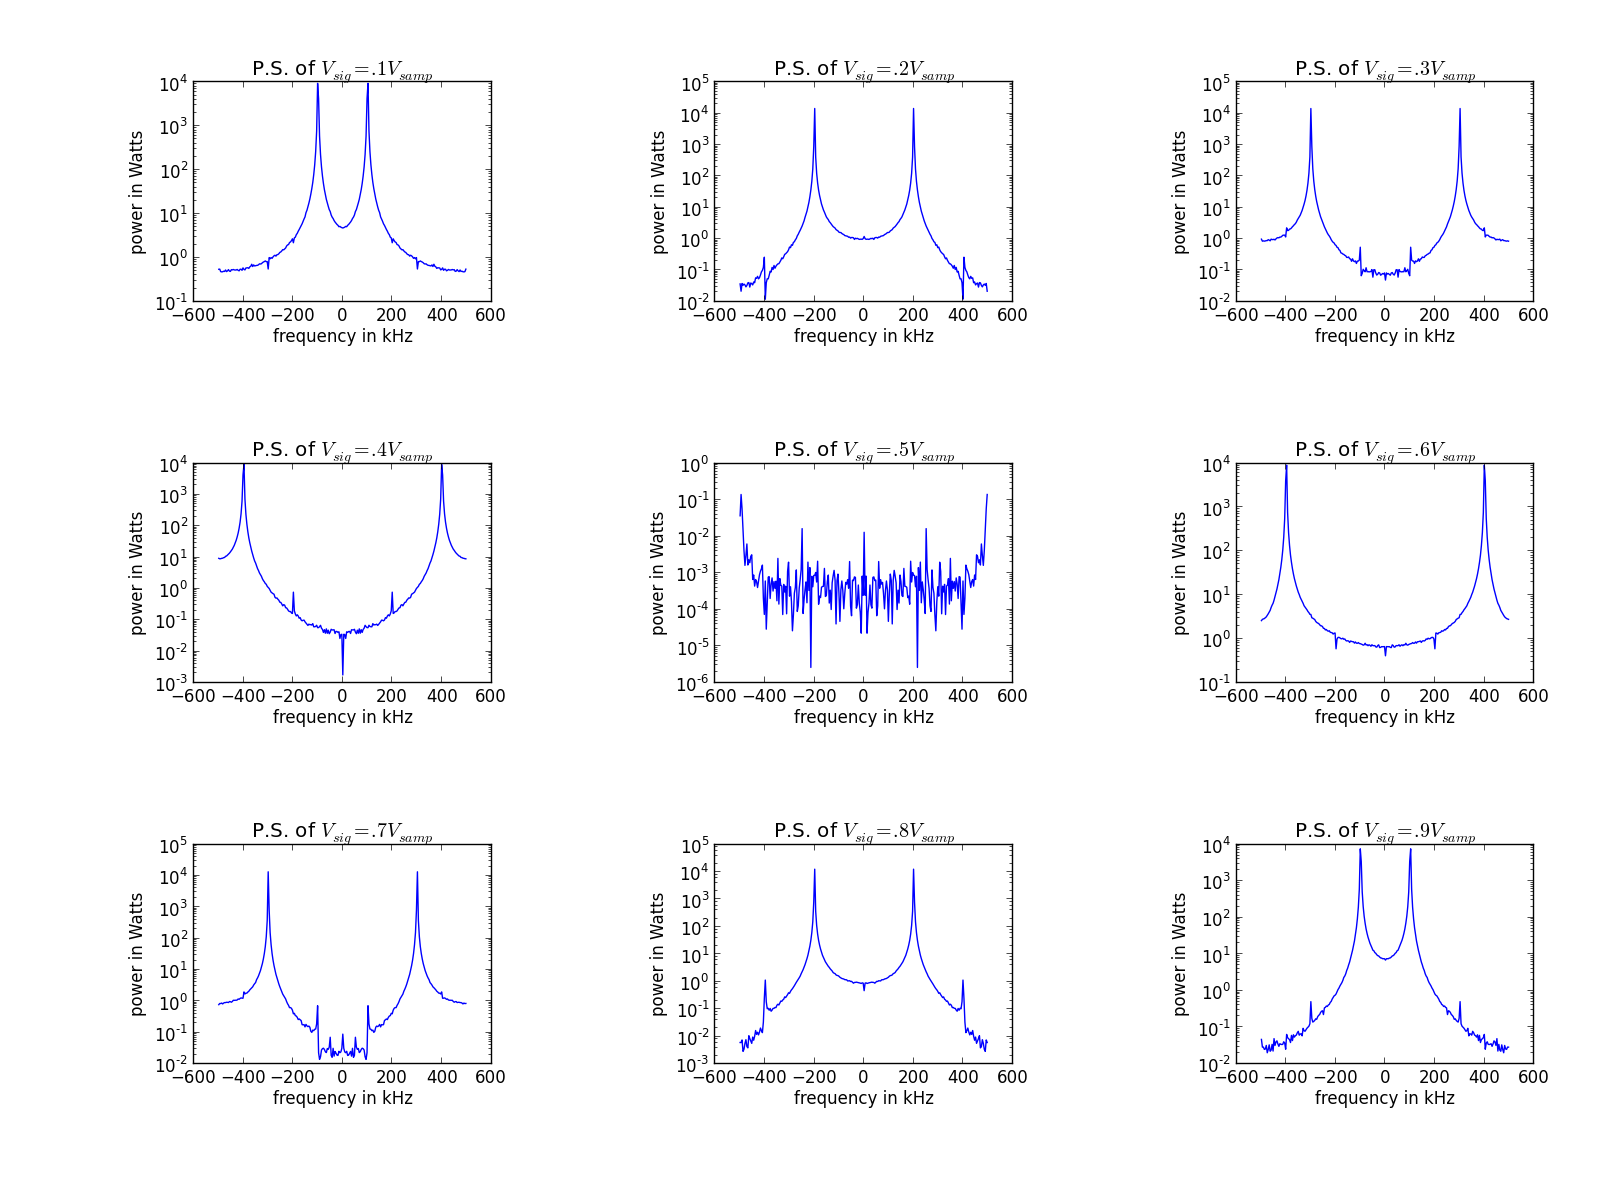
\includegraphics[scale=0.4]{DFTplotslog.png}
\caption{the leakage power shown as the 'fringe' peaks}
\label{DFTplotslog}
\end{figure}
This is the result of the signal in the time domain resulting in a
convolution in the frequency domain. The small spikes that are seen are
the leakage, showing up further away from the spectral peaks, those
small spikes are not perfectly periodic in the Fast Fourier
Transform. frequency bins are just the number of samples you decide to
take over the sample frequency, here, there are two waves mixed
together, these waves are periodic (being sine waves) and so when
there's is a linear combination of them, within that bin one wave will
fit in it while the other's wavelength will not fit within the bin and
so a bit of it `leaks' into the next bin, and so that is what is seen in
the above graph. 

\subsection{Frequency Resolution}

In regards to spectral resolution, it is defined as the siganl frequency
over the number of data points you have. So, you could have the spikes
be very close to gether, achieving very high resolution, but this takes
alot of resources from the computer, slowing down your data collection
time. We can't get infinite resolution because of limitations on our
current hardware. To sample at rates good enough for our purposes, all
we want is to stay near the Nyquist critereon,  or have a signal
frequency smaller than the sample to get adequate results. 

\section{Working with the ROACH}

\subsection{Methods}
During the course of this week of the lab, Isaac Domalgalski developed
the code to take the data the rest of the group needed. All other work
henceforth all data that was worked with came from his code. This report
used and mainpulated that data. 

\subsection{DSB Mixer Power Spectra}
Having plotted the power spectrum of the sum and difference cases versus
frequency we get this plot
\begin{figure}[H]
\center
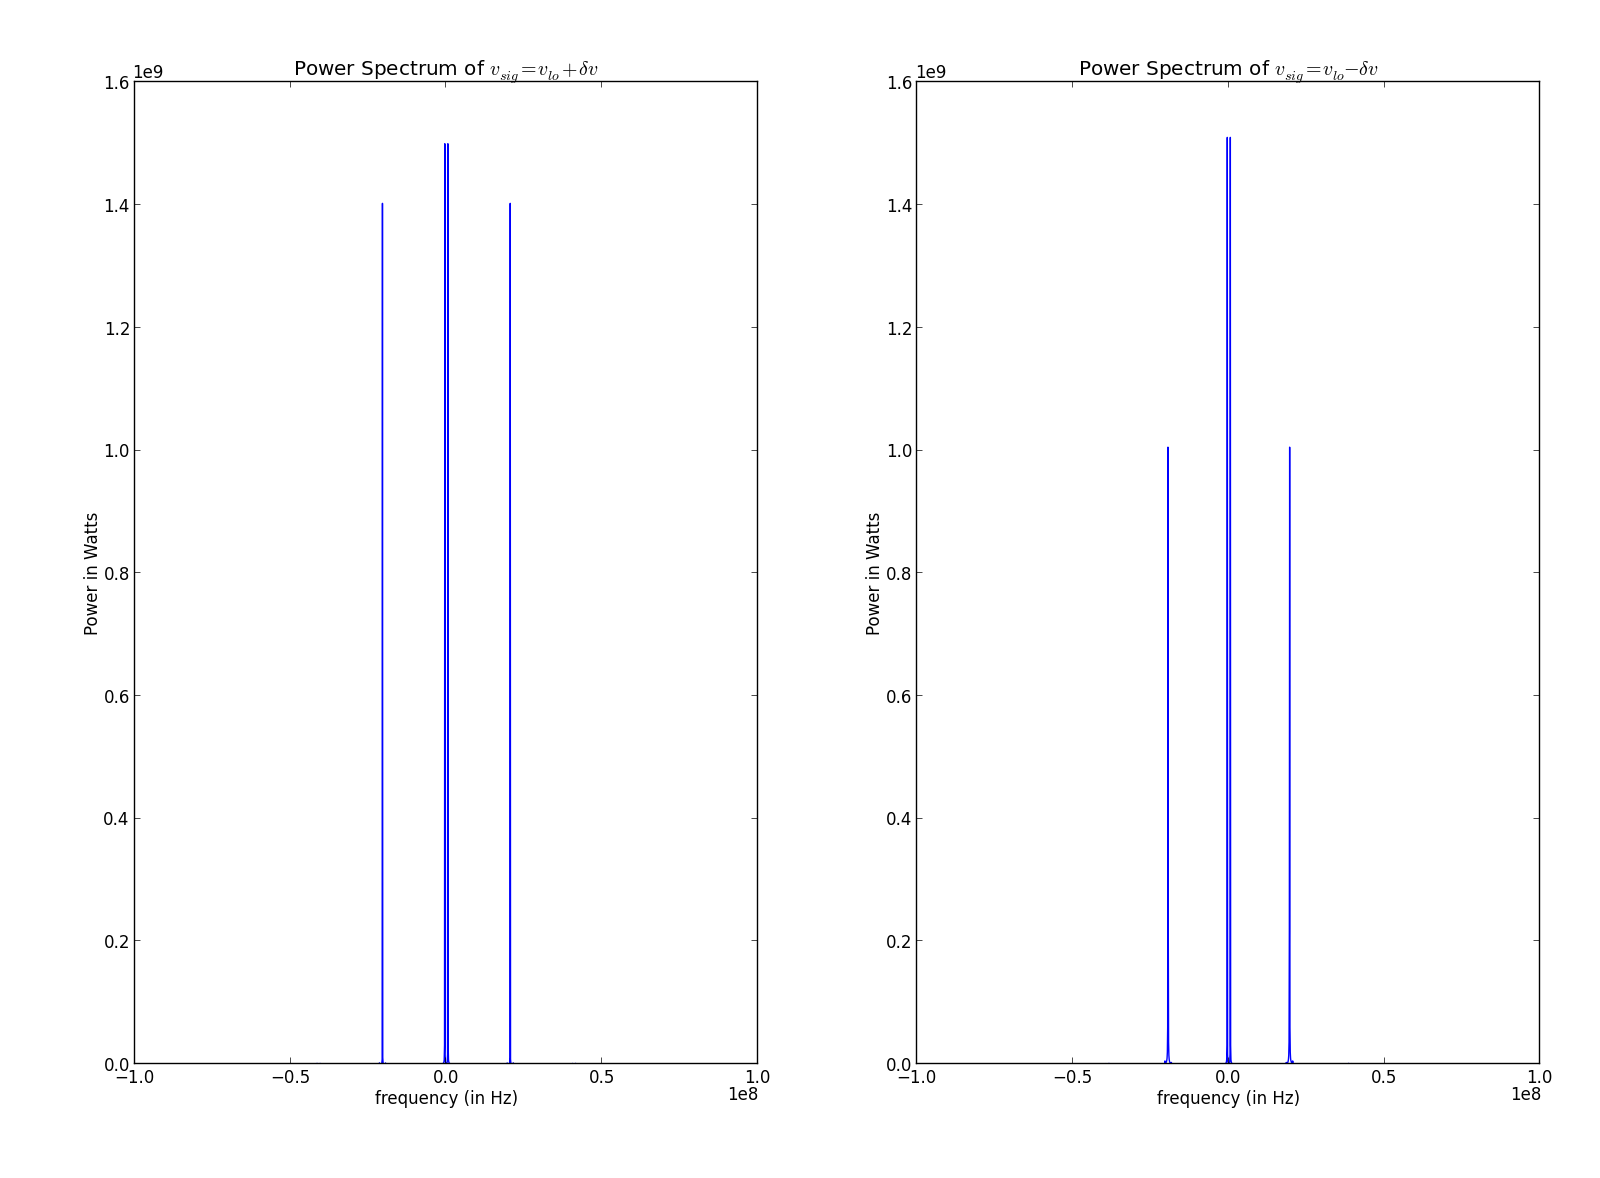
\includegraphics[scale=0.4]{powerspectmixed.png}
\caption{The power spectra for $\pm \delta v$.}
\label{powerspectmixed}
\end{figure}
An interesting thing that we see in these spectra is that the middle
`thick' line is actually two lines very close together which confirms
the presence of two waves that been mixed together into one sine
wave. Now, the upper sidebands refer to the bands (spikes) which are on
the positive side of the x-axis(frequency); the real part of the sine wave. Whereas
the lower sidebands refer to those on the negative x-axis; they
correspond to an imaginary part of the sine wave. 

We see the waveforms as pictured below,  and we will focus on the
$v_{sig} = v_{lo} + \delta v$ From observations made that day, it did
look like what was seen on the oscilloscope's trace.
\begin{figure}[H]
\center
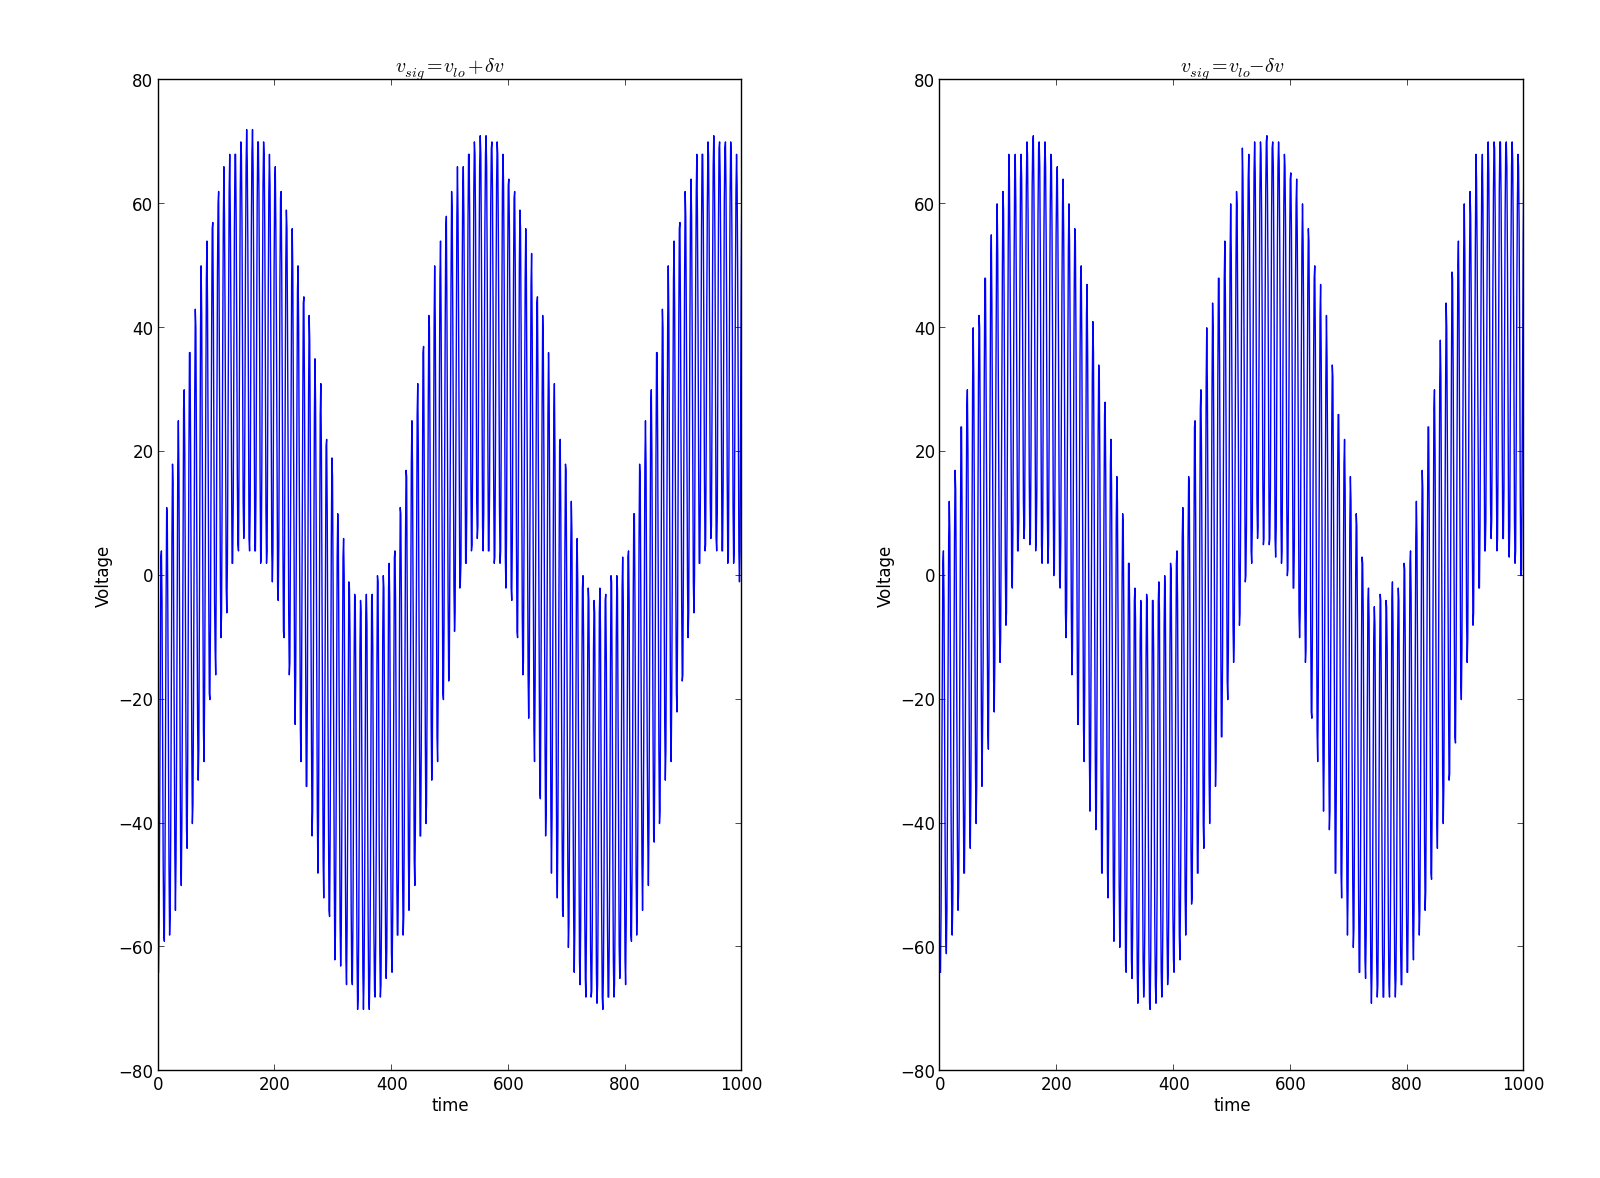
\includegraphics[scale=0.4]{mixedsignals.png}
\caption{the Wave form of both mixed signals}
\label{mixedsignals}
\end{figure}
 Taking the Fourier
Transform and zeroing out the sum frequency we then apply the inverse
fourier transform on it and we retrieve a new signal

\begin{figure}[H]
\center
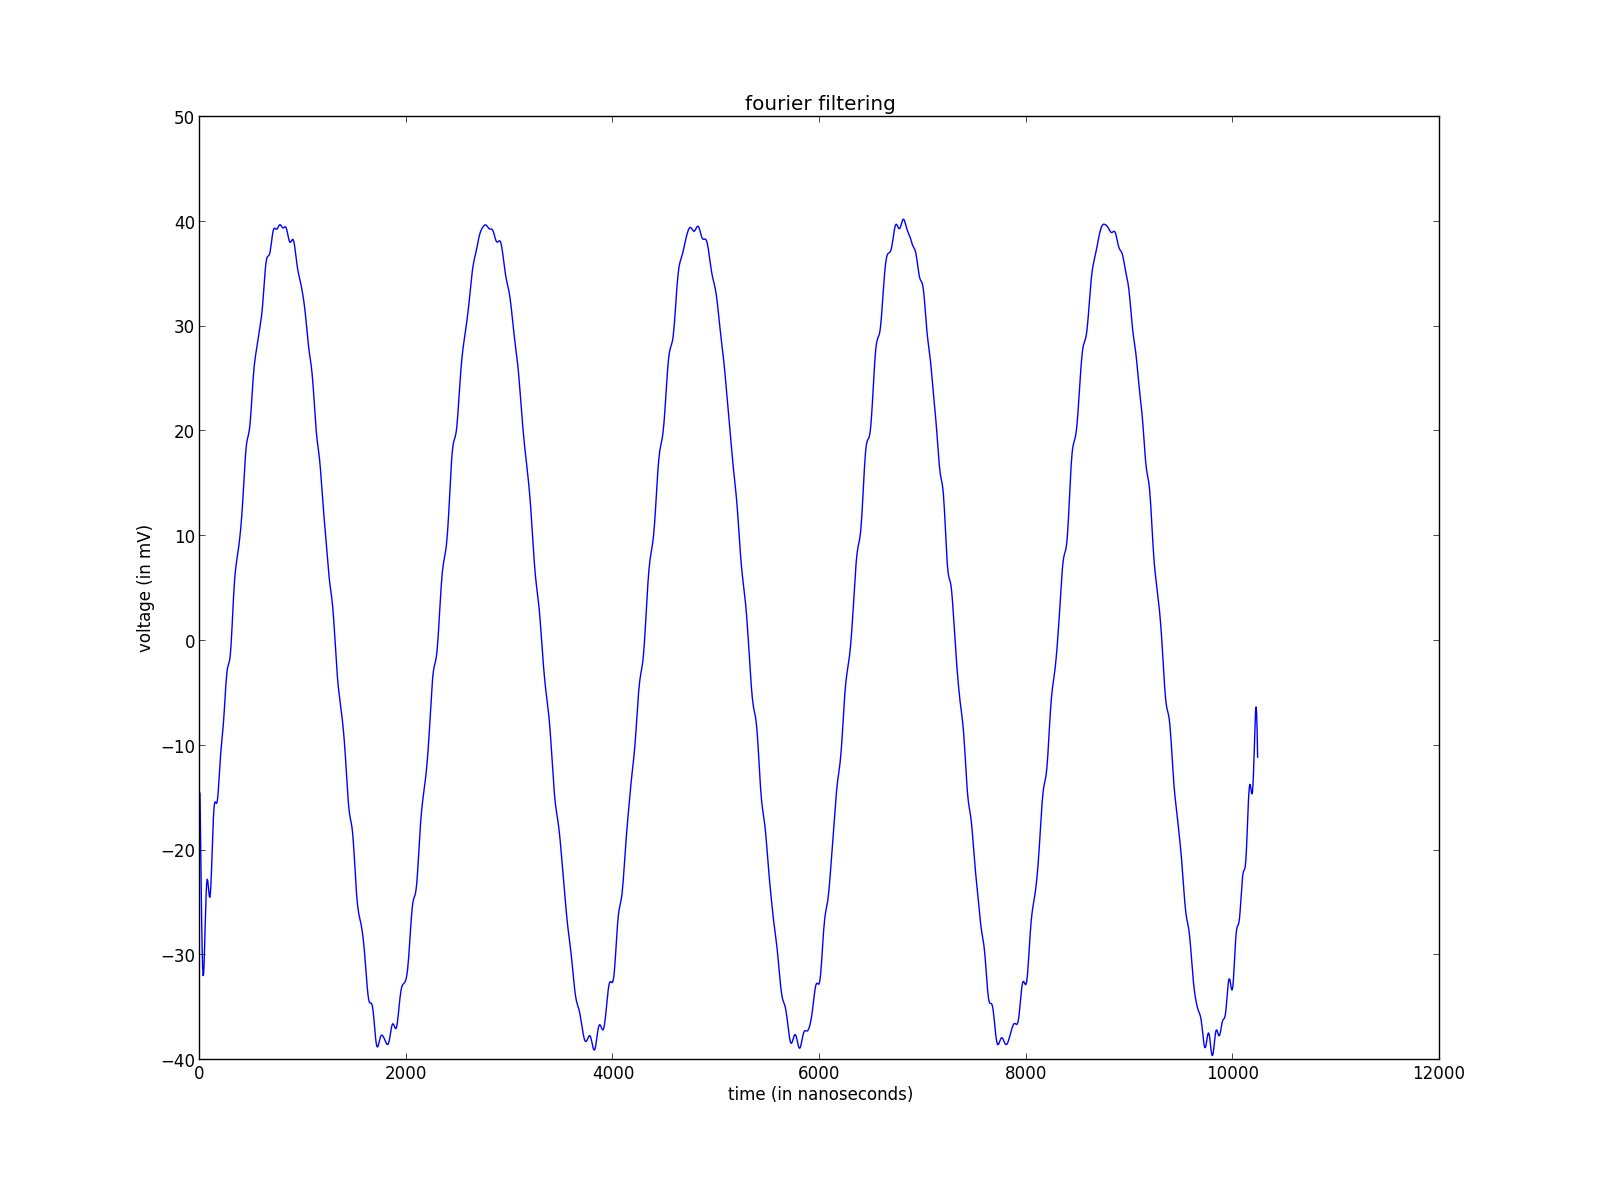
\includegraphics[scale=0.4]{fourierfiltering01.png}
\caption{the original wave after zeroing and inverse fourier transforming}
\label{fourierfiltering01}
\end{figure}
This new signal is $\delta v$ the difference of $v _{sig}$ and $v_{lo}$
by zeroing out the sum after fourier transforming the waveform, we
effectively destroyed the mixed wave. This new wave is the output of the
mixer without the higher frequency part that was originally mixed in. 


\subsection{Digital Mixing and Power Spectra}
So now, for the digital and analog power spectrum DSB mixing cases, we
see,
\begin{figure}[H]
\center
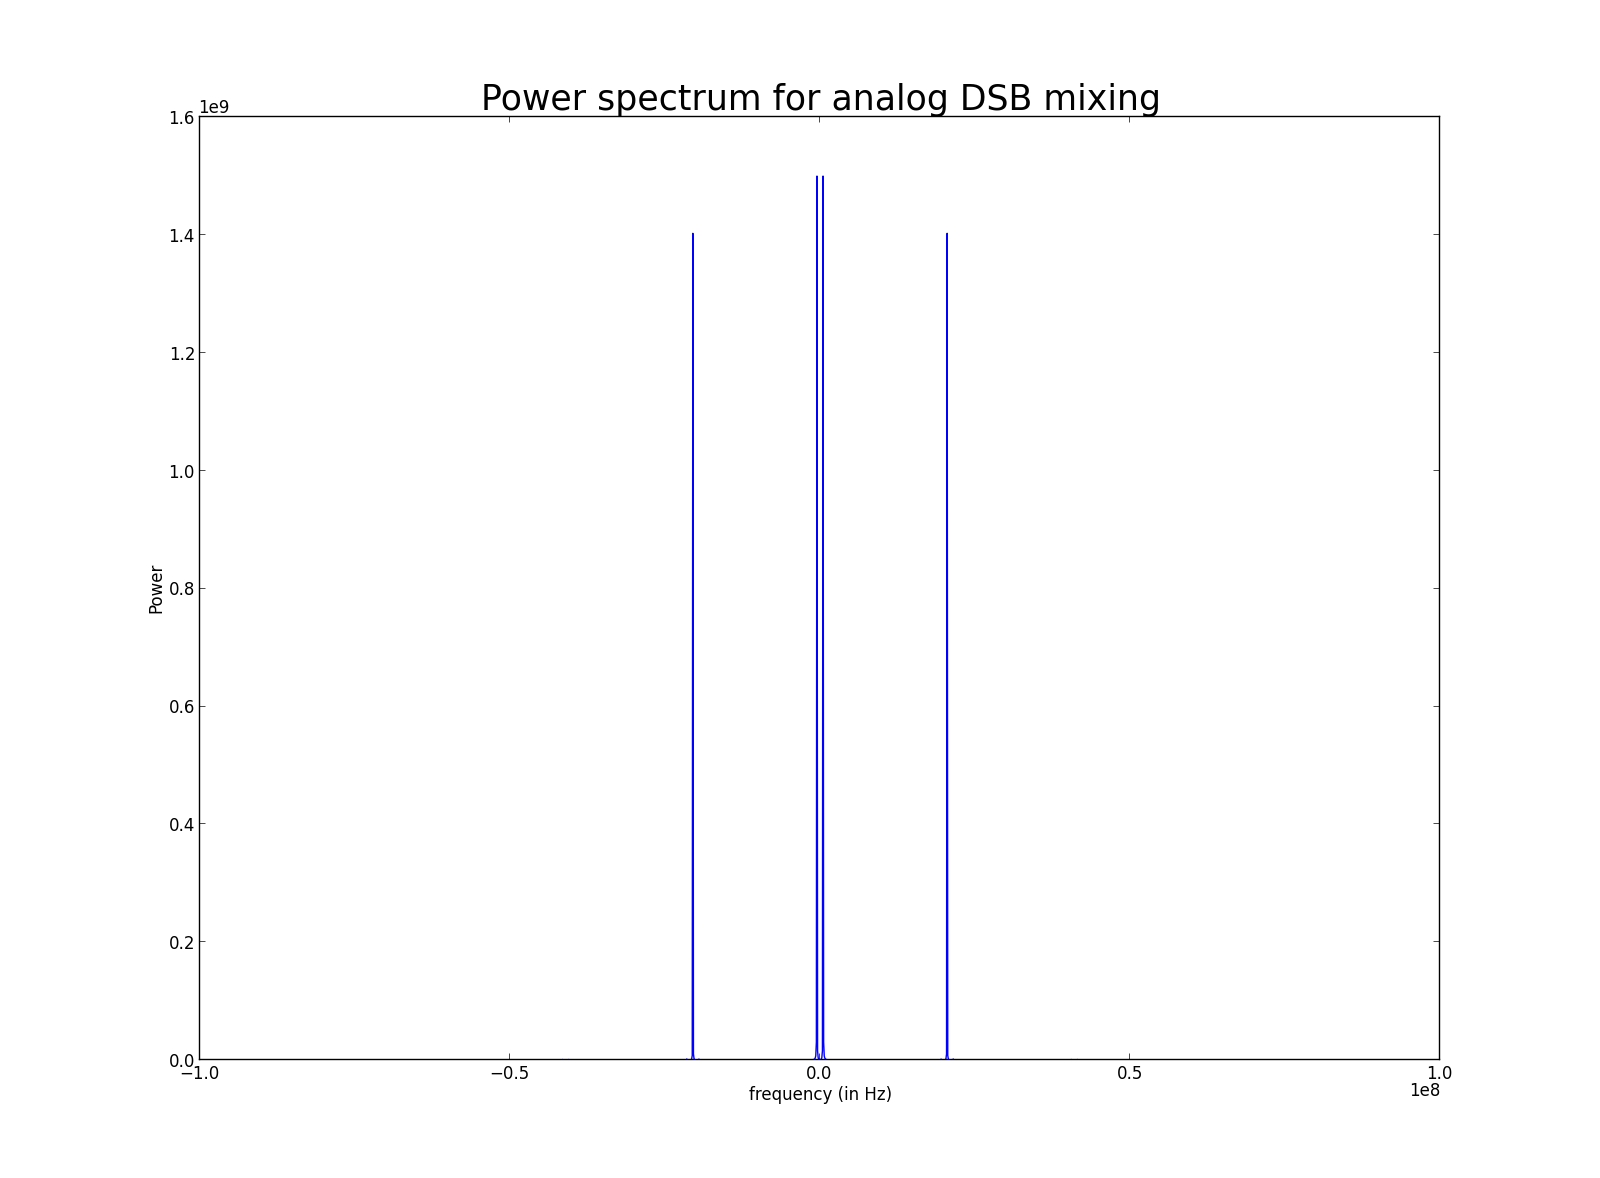
\includegraphics[scale=0.4]{powerspectanadigdsbmix.png}
\caption{The power Spectrum of the analog DSB mixer}
\label{anadsb}
\end{figure}
followed by the digital version
\begin{figure}[H]
\center
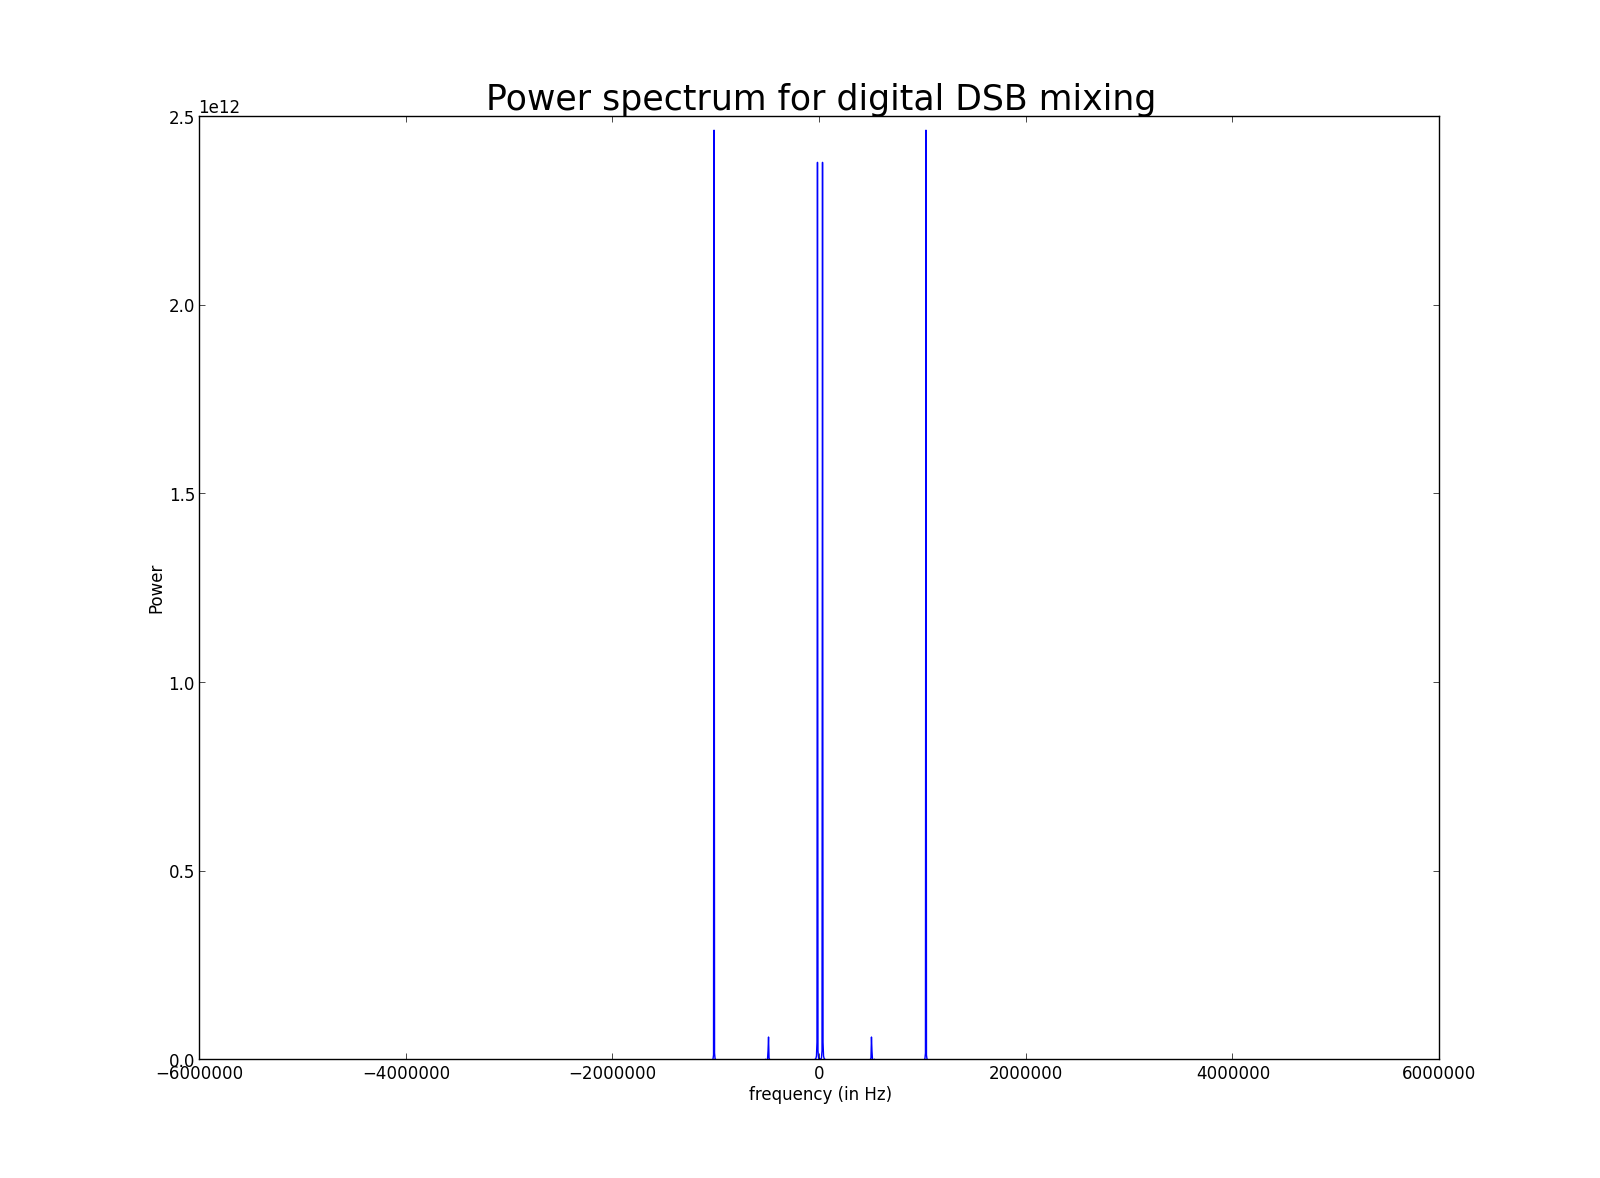
\includegraphics[scale=0.4]{powerspectdigdsbmix.png}
\caption{The power Spectrum of the digital DSB mixer}
\label{digdsb}
\end{figure}
The main diffence between these two plots is the DC offput observed in figure
\ref{digdsb} which is the result of the waves not being perfectly
centered on 0 volts when being mixed digitally. Another difference in
the graphs that is noticed is the scaling of the x-axis,  the reason for
this was the sampling frequency that was used, in the analog case, 200
MHz was used whereas the digital version used 20 MHz as the sampling
frequency, thus why the x-axis is off by a factor of 10. The Waveform of
the digital mixing case looks like 

\begin{figure}[H]
\center
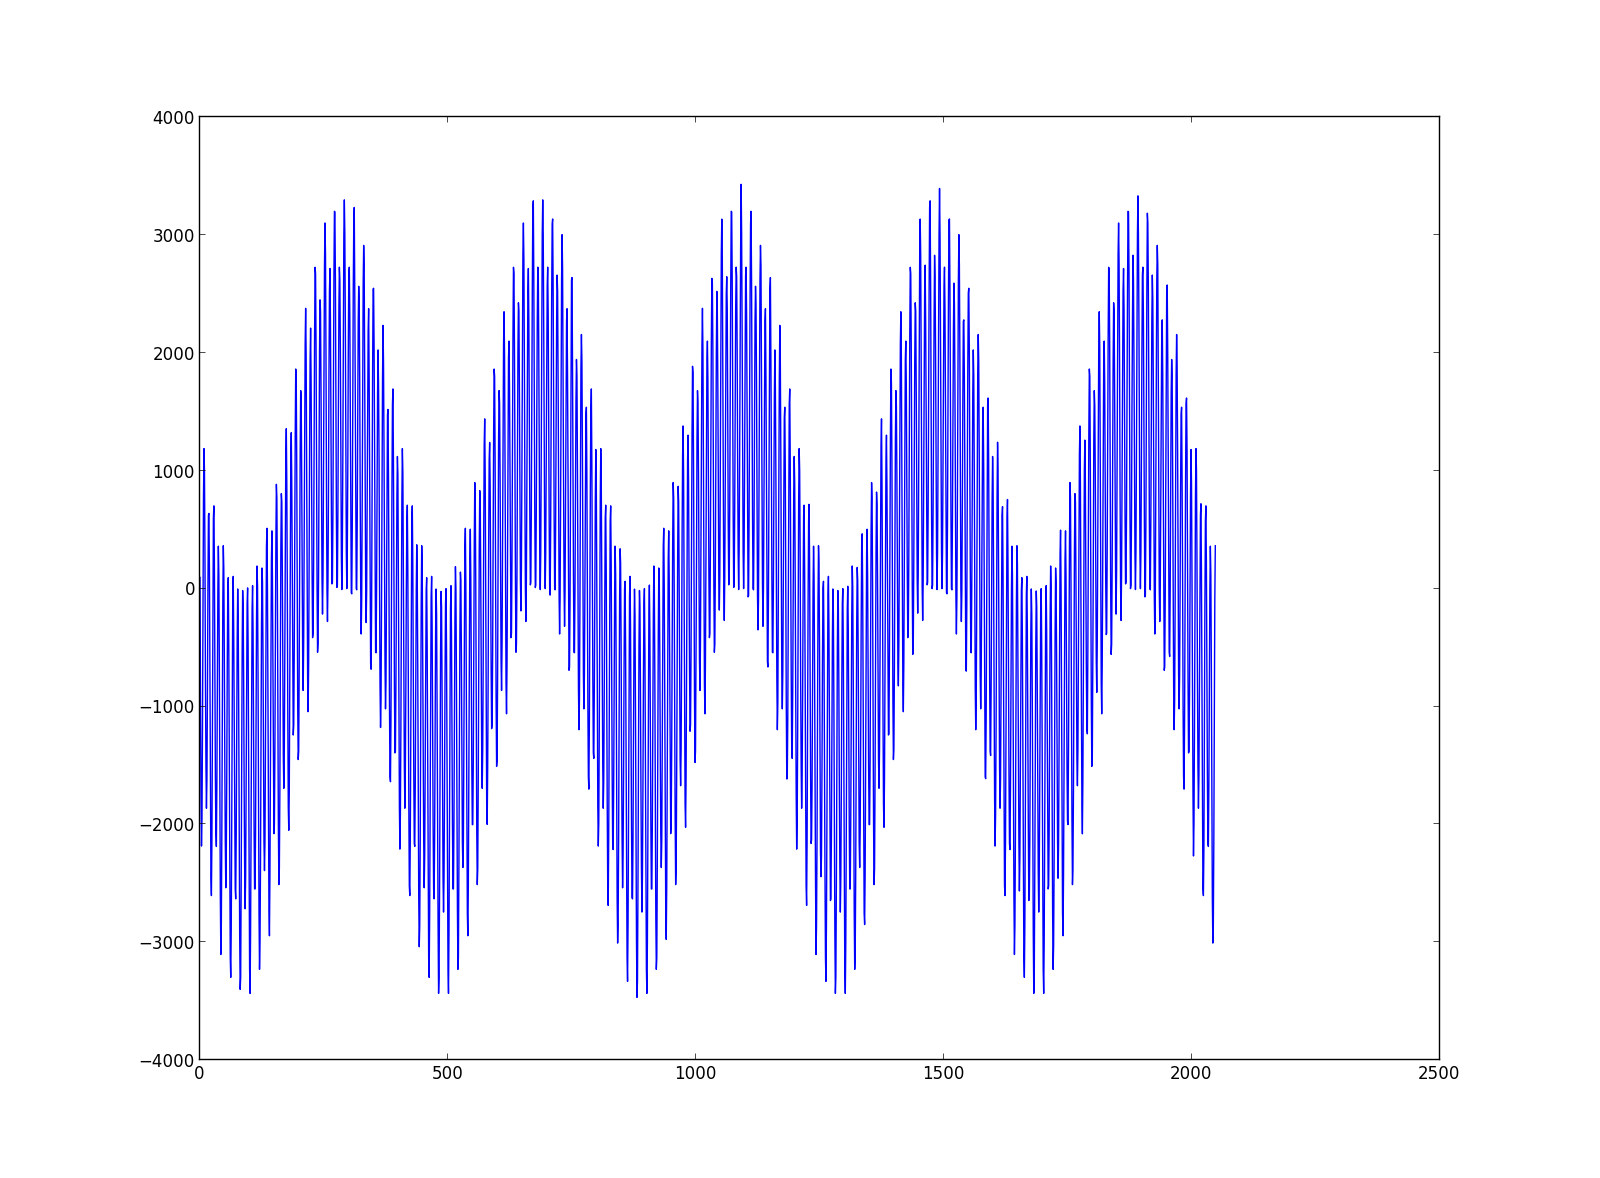
\includegraphics[scale=0.4]{digmixdsbwaveform.png}
\caption{The Waveform of the digital DSB mixer}
\label{wavedsb}
\end{figure}
Here the waveform is plotted as a function of voltage versus time, this
waveform includes the mixed signals we input.


Now we look at the power spectrum of the SSB mixer 

\begin{figure}[H]
\center
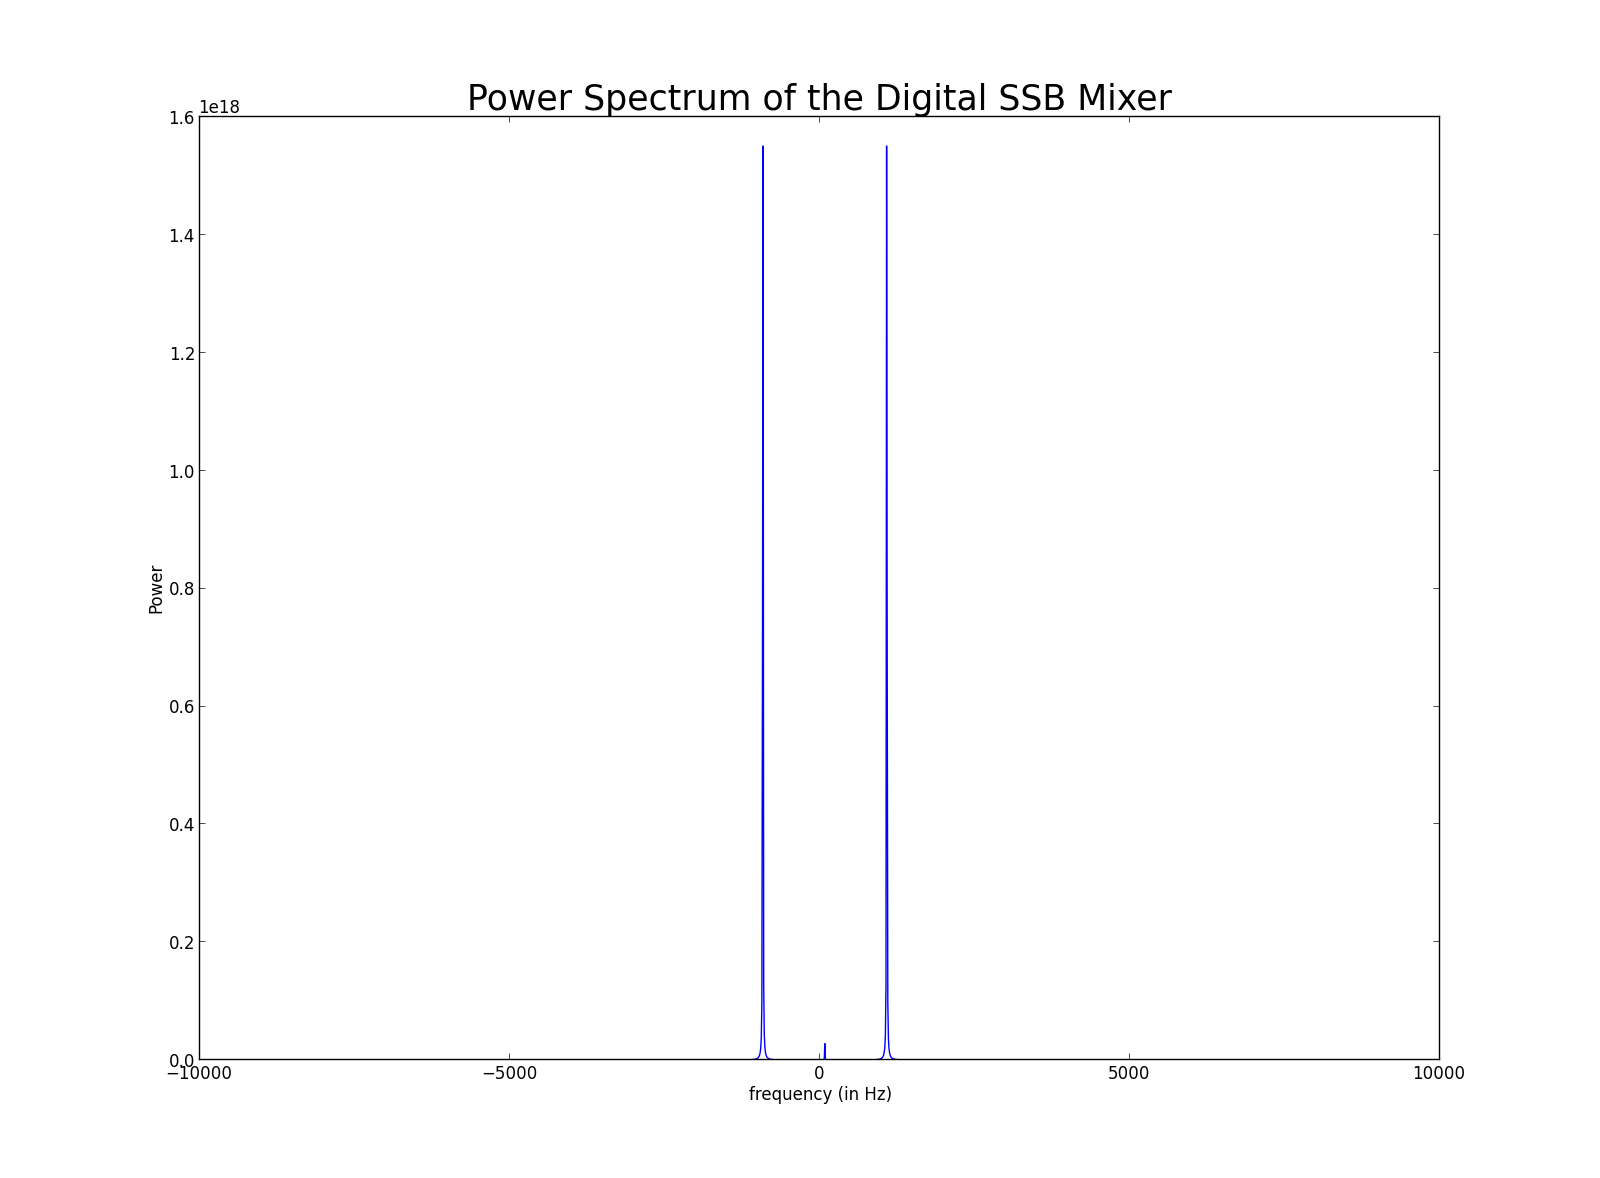
\includegraphics[scale=0.4]{powerspectdigssbmix.png}
\caption{The power Spectrum of the digital SSB mixer}
\label{digssb}
\end{figure}
The reason the graph now looks like this is because the wave consisted
of a real and imaginary part. When taking the power spectrum we needed
to square the absolute value of the Linear combination of the cosine and
sine components of the wave,  with the sine component multiplied by the
imaginary number, i because the power spectrum must be real. This
multplication by i then forces the spikes to shift a liitle bit to the
right, thus why the graph is shifted positively.

\begin{figure}[H]
\center
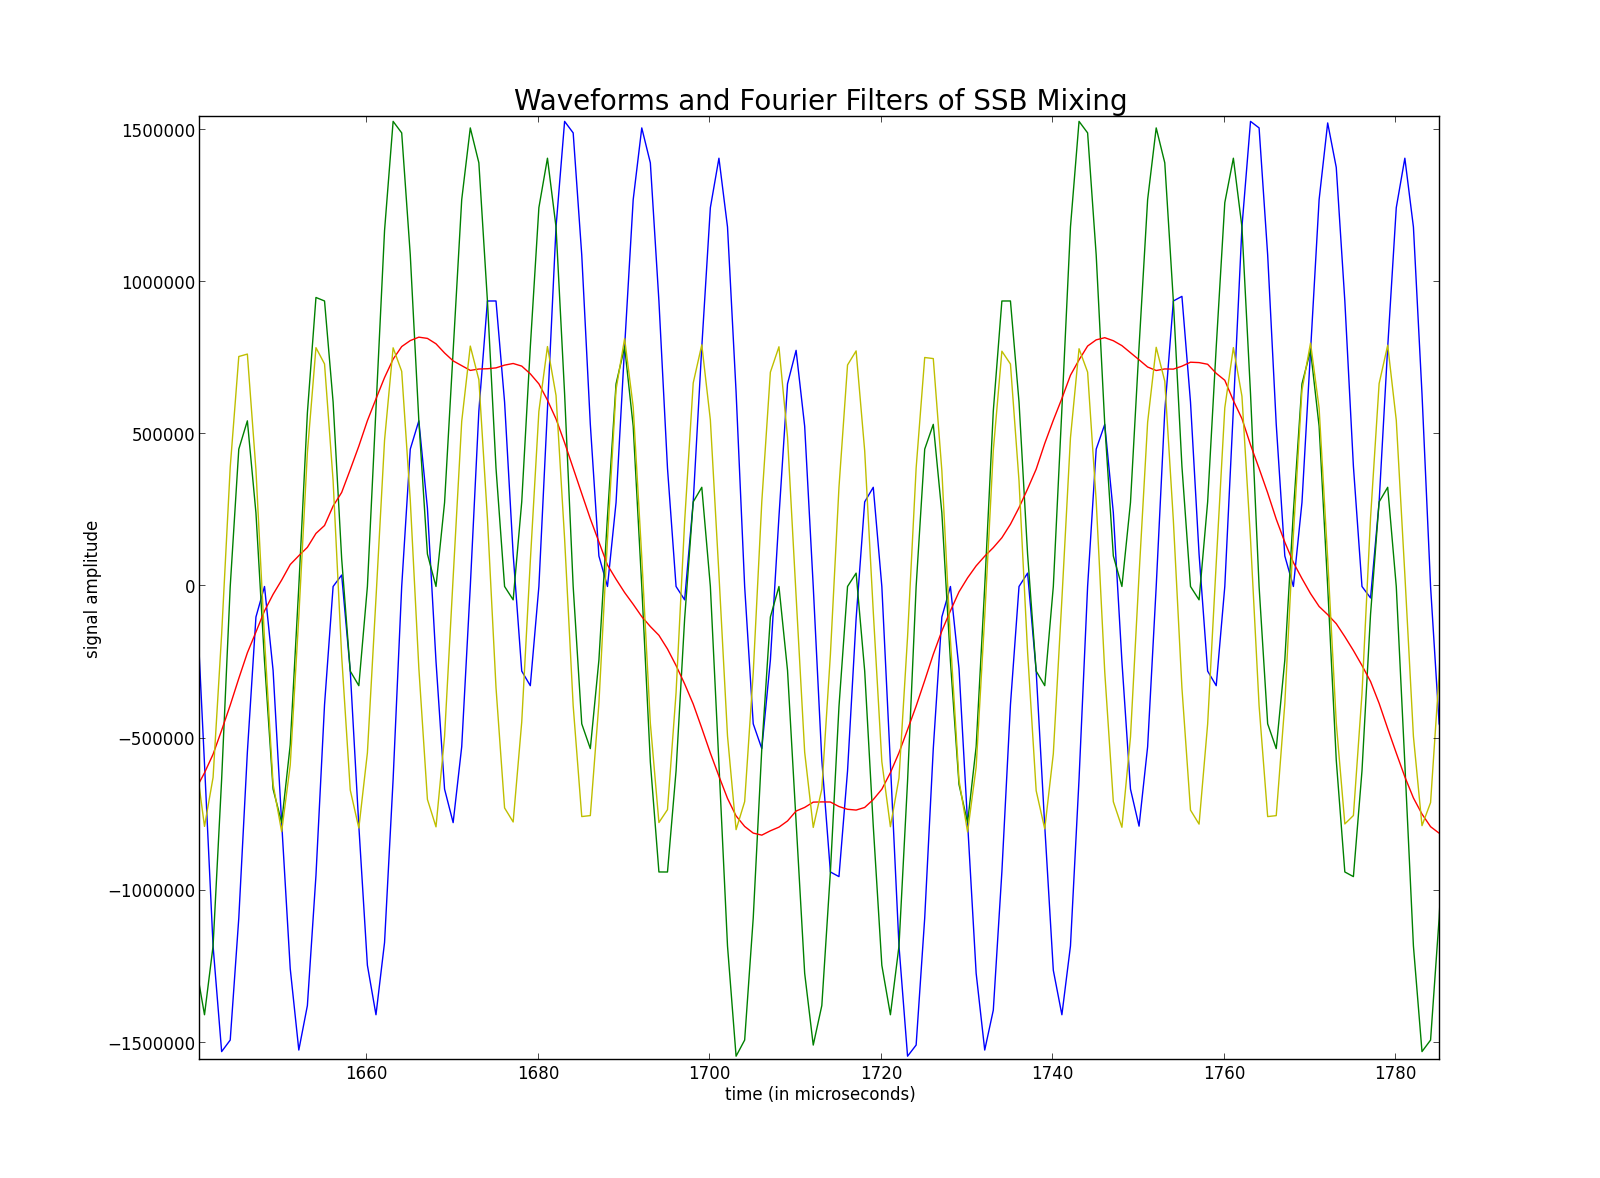
\includegraphics[scale=0.4]{waveformssbdig.png}
\caption{The Waveform and tones of the imaginary and real parts of the wave}
\label{waveformssb}
\end{figure}

Here, we present the waveform of the sine and cosine waves. The blue
wave represents the cosine wave and the gren represents the sine waves
which lags behind the cosine wave by a liitle bit. The red wave
represents the tone we are looking for when the spike in frequency
domain is zeroed out for the imaginary part of fourier transform and
then inverse fourier transformed, so we see that this tone has a
negative frequency since the previous power spectrum was offset
positively. 

In implementations of DSB and SSB mixing, we see that when we use DSB
mixing,  we get bands the lower and upper bands whereas in the SSB
mixing we can only get either one or the other depending on the cosine
and sine components of digital waves. If the cosine and sine waves were
out out phase, we would expect to see errors in our power spectrum,
mainly some spectral leakage.

\section{Coefficients and Digital Down Conversion}
In this section coefficients for the Finite Impulse Response filter will
be calculated. 
FIR filters implement frequency domain filters with a tunable shape determined
by those same coefficients that convoolve with an input wave form. In
this experiement, an input wave of 20 MHz was chosen out out a series of
other input waves.  A diagram of a FIR filter is displayed below.
\begin{figure}[H]
\center
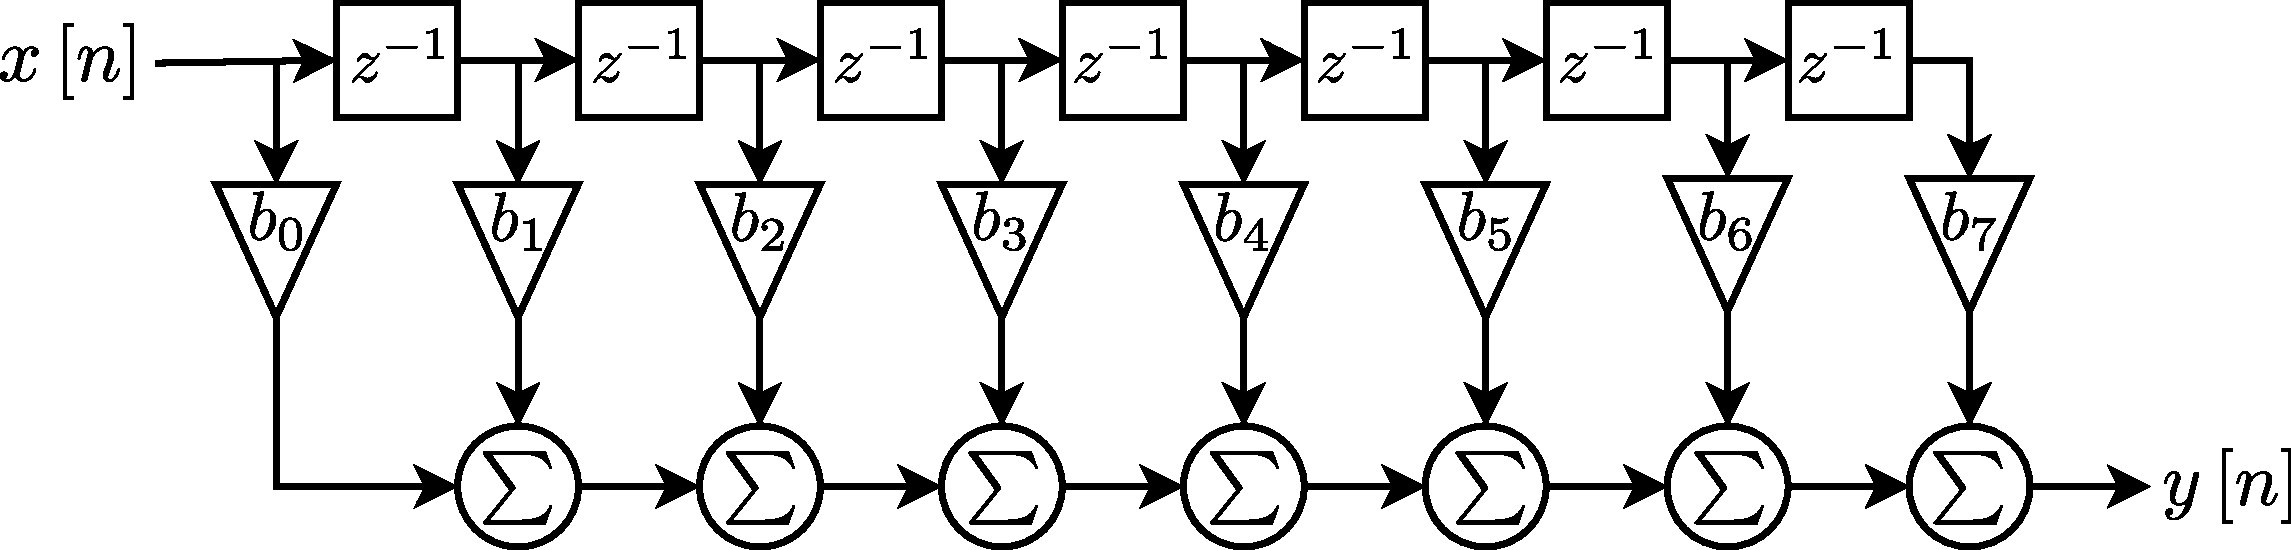
\includegraphics[scale=0.4]{fir-filter.pdf}
\caption{A digram of the FIR filter}
\label{fir-filter}
\end{figure}
 Some signals x[n] propagate through the chain of delays, represented by
 the $z^{-1}$ boxes.  At each clock, N samples are multiplied by N
 coefficients $b_{o}...b_{N-1}$ and summed. 

\subsection{Coefficients of the FIR Filter}
Below we see the calclated coefficients of the FIR filter for an imput
siganl of 20 MHz.

\begin{table}[H]
\center
\begin{tabular}{|c|c|}
\hline
\multicolumn{2}{|c|}{Coefficients for the FIR filter}\\
\hline
Floating Point & Fixed Binary \\
\hline
$0.125$ & $0.00100000000000000$ \\
\hline
$-0.0517730712890625$ & $1.11110010101111110$ \\
\hline
$-0.125$ & $1.11100000000000000$ \\
\hline
$0.3017730712890625$ & $0.01001101010000010$ \\
\hline 
$0.625$ & $0.10100000000000000$ \\
\hline
$0.317730712890625$ & $0.01001101010000010$ \\
\hline
$-0.125$ & $0.11100000000000000$ \\
\hline
$-0.0517730712890625$ & $1.11110010101111110$ \\
\hline
\end{tabular}
\caption{the coefficients used for digital down converting. We can see
  the sum of 32 bits on the binary fixed point column}
\label{coef table}
\end{table}
 when we pad out our expected coefficients with an array of 52 zeroes,
 we want to create a plot of desired bandpass filter, by concatenating
 an array of [1,1,1,0,0,0,1,1] with these zeroes then fourier
 transforming we get an ideal plot of 

\begin{figure}[H]
\center
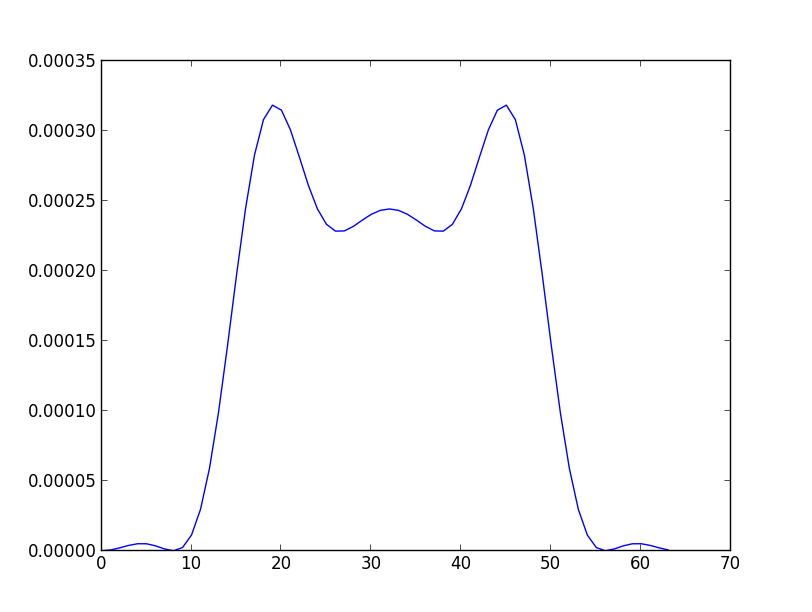
\includegraphics[scale=0.4]{desiredbandpass.png}
\caption{The desired bandpass we would like}
\label{bandpass}
\end{figure}
 this is the ideal shape we would want for this filter.

\subsection{The Filter shape}
There wasn't enough time to get the plots for this section of the lab.
The true shape of the filter should not match up with the ideal one we
calculated above, noise would distort the graph somewhat.


\section{Conclusion/Discussion}
Sampling with a signal is imporatnt in the field of astronomy because we
want to have the minumum data to analyze various things in astronomy for
practical reasons, computer space. Analyzation involves being able to
resolve signals. There are still some things that are not understood at
this end for instance, the whole of week 3, but mixing of signals and
looking at their power spectra, waveforms is understood better 


\end{document}